% %% %%%%%%%%%%%%%%%%%%%%%%%%%%%%%%%%%%%%%%%%%%%%%%%%%%%%%%%%%%
% intro-triac.tex
%
% Author:  Mauricio Matamoros
% License: MIT
%
% %% %%%%%%%%%%%%%%%%%%%%%%%%%%%%%%%%%%%%%%%%%%%%%%%%%%%%%%%%%%
%!TEX root = ../practica.tex
%!TEX root = ../references.bib

% CHKTEX-FILE 1
% CHKTEX-FILE 13
% CHKTEX-FILE 46

\subsection{TRIACs}%
\label{seq:intro-triac}

Un TRIAC o triodo interruptor para corriente alterna (\emph{Triode AC Switch}) es un integrado de estado sólido compuesto por dos tristores conectados en paralelo inverso (véase~\Cref{fig:triac-analogy}) que permite conmutar la corriente que pasa por un circuito de AC a alta frecuencia de manera similar a como operan los transistores bipolares y FETs en DC.
Es decir, un TRIAC es un interruptor de estado sólido que puede operar a gran velocidad que, a diferencia de los relés, no existe la posibilidad de que un arco eléctrico funda los metales y el dispositivo se quede en encendido permanente, sino que al quemarse un TRIAC siempre abre el circuito.
Por otro lado, basta una corriente muy pequeña entre el gate ($G$) y cualquiera de las terminales ($MT_1$ y $MT_2$) para encender al TRIAC, lo que lo convierte en el aliado ideal para controlar dispositivos de alta potencia con un microcontrolador.

\begin{figure}[H]
	\centering
	\begin{subfigure}{0.3\linewidth}
		\centering
		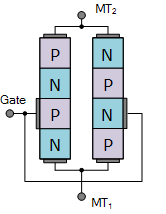
\includegraphics{img/triac1.png}
		\caption{Construcción física}%
		\label{fig:triac-construction}
	\end{subfigure}
	\begin{subfigure}{0.3\linewidth}
		\centering
		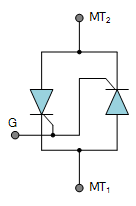
\includegraphics{img/triac2.png}
		\caption{Equivalente en tristores}%
		\label{fig:triac-analogy}
	\end{subfigure}
	\begin{subfigure}{0.3\linewidth}
		\centering
		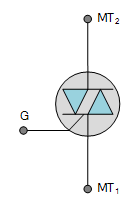
\includegraphics{img/triac3.png}
		\caption{Símbolo}%
		\label{fig:triac-symbol}
	\end{subfigure}
	\caption[Triac]{El Triac\footnotemark{}}%
		\label{fig:triac}
\end{figure}
\footnotetext{Fuente de imagen: \url{https://www.electronics-tutorials.ws/power/triac.html}}

Como siempre, al utilizar un TRIAC es deseable aislar la parte de corriente directa del circuito de la parte de corriente alterna, es decir, el TRIAC deberá estar aislado pero acoplado al circuito DC.
Esto normalmente se realiza mediante el uso de optoacopladores tipo MOC, tal como se ilustra en la \Cref{fig:triac-circuit}.

\begin{figure}[H]
	\centering
	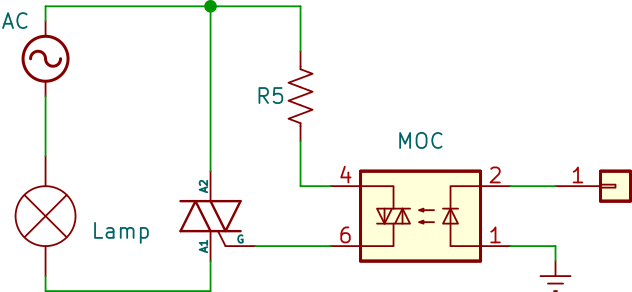
\includegraphics[width=0.5\textwidth,height=5cm,keepaspectratio]{img/triac-circuit.png}
	\caption{Triac optoacoplado}
	\label{fig:triac-circuit} %chktex 24
\end{figure}

Una peculiaridad de los TRIAC es que el tiempo de encendido no es proporcional al tiempo que se inyecta una corriente por el \emph{gate}, sino que una vez recibido el pulso de arranque el TRIAC permanecerá habilitado hasta el siguiente cruce por cero de la onda senoidal de corriente alterna.
Es decir que, diferencia de los transistores de juntura bipolar (BJT) o de efecto de campo (FET), un TRIAC no puede usarse para modular corriente directa con un PWM.
Por este motivo es necesario utilizar el \textbf{complemento} del ángulo de fase al modular la potencia de un dispositivo usando un TRIAC.

Por ejemplo, supóngase que se desea obtener el 50\% de potencia\footnotemark{} de una resistencia,
considerando que una resistencia tiene una respuesta lineal (el voltaje y la corriente están en fase) y que la senoidal de la línea de AC es una simétrica.
% el ángulo de disparo $\phi$ sería de $\phi = \frac{\pi}{2}$.

\begin{align*}
	% \frac{V_{P}}{2} = &
	% V_{P} \cdot \sin\left(2\pi \cdot f \cdot t\right) \\
	\cancel{V_{P}} = &
	\cancel{V_{P}} \cdot \sin\left(2\pi \cdot f \cdot t\right) \\%
	%
	1 = &
	\sin\left(2\pi \cdot f \cdot t\right) \\%
	%
	\arcsin\left(1\right) = &
	\cancel{\arcsin}\left(\cancel{\sin}\left(2\pi \cdot f \cdot t\right)\right) \\%
	%
	\frac{\pi}{2} = &
	2\pi \cdot f \cdot t\\%
	%
	t = &
	\frac{\frac{\cancel{\pi}}{2}}{2\cancel{\pi} \cdot f} \\%
	%
	t =& \frac{1}{4f}
\end{align*}

Si la frecuencia de línea fuera de 50Hz, el tiempo de disparo $t_{50\%}$ después del cruce por cero sería:

\begin{align*}
	t_{50\%} =& \frac{1}{4 \times 50\text{Hz}} \\
	=& \frac{1}{200\frac{1}{s}} \\
	=& 0.005s \\
	=& 5ms \\
\end{align*}

De acuerdo con lo anterior, el triac deberá encenderse en $t=5ms$ y así permanecerá encendido hasta que el voltaje de la línea pase por cero y se invierta, es decir, la mitad del ciclo.
Ni siquiera es necesario mantener la señal de encendido del TRIAC durante este tiempo.
Para encender el triac basta con un breve pulso normalmente despreciable (ej.~$10\mu s$).

% En contraste, si la señal de habilitación de se encendiera en $t=0$ y apagarse en $t=5ms$; sin embargo, tal como se mencionó anteriormente, si el TRIAC se enciende en $t=0$ éste permanecerá encendido durante todo el ciclo

\footnotetext{
	Como $P=VI$ y $V=RI$ entonces $P=\frac{V^{2}}{R}$ donde $V$ es el voltaje promedio o RMS suministrado.
	Aquí es necesario hacer una distinción entre el voltaje RMS nominal de línea $V_L$ y el voltaje RMS de la onda recortada por del TRIAC $V_\alpha$, pues la potencia suministrada se corresponderá con este último de la forma:
	\begin{equation}
	\label{eqn:va}
		V_\alpha = V_L\sqrt{
			\frac{1}{\pi}
			\left(
				\pi - \alpha +
				\frac{\sin\left(2\alpha\right)}{2}
			\right)
		}
		\text{ ; donde } \alpha=\omega t
		\text{ y } \omega = 2\pi f
	\end{equation}

	Cuando lo que interesa es un percentil de la potencia suministrada se tiene que
	$P_\text{\textsc{Max}} = P_L = P_{\alpha=0}$,
	por lo que se puede utilizar el cociente
	$\frac{P_\alpha}{P_L} = \frac{V_\alpha^{2}\cancel{R}}{V_L^{2}\cancel{R}}$ que, despejando en la \Cref{eqn:va} produce:

	\begin{equation}
	\label{eqn:pa}
		P\% = \left(
			1 - \frac{\alpha}{\pi} +
			\frac{\sin\left(2\alpha\right)}{2\pi}
		\right) \times 100
	\end{equation}

	Que, a una frecuencia de 50Hz y con $t=5ms$ ($\alpha=0.5\pi$) reporta un 50\% de potencia.

	Es importante remarcar que la \Cref{eqn:pa} es válida sólo si la impedancia de la carga es invariante en el tiempo ($\frac{dR}{dt}=0$).
	Si este no fuere el caso (como por ejemplo con una lámpara incandescente) la potencia no variará de forma cuadrática proporcional con el voltaje.
}

